\documentclass[12pt, a4paper]{article}

% PRÉAMBULE -------------------------------------------------------------------

\usepackage[utf8]{inputenc}
\usepackage{textcomp}
\usepackage{tikz}
\usepackage{amsmath}
\usepackage{amsfonts}
\usepackage{graphicx}
\usepackage[T1]{fontenc}
\usepackage[french]{babel}

\title{Projet ISN - Terminale S - Démineur}

\author{BOURGET Alexis, LE TERTE Dorian, MIGADEL Kevin - TS1}

\date{Année Scolaire 2015-2016}

% --------------------------------------------------------------- FIN PRÉAMBULE

\begin{document}

\pagenumbering{gobble} % Pas de numéro sur la première page
\maketitle
\centerline{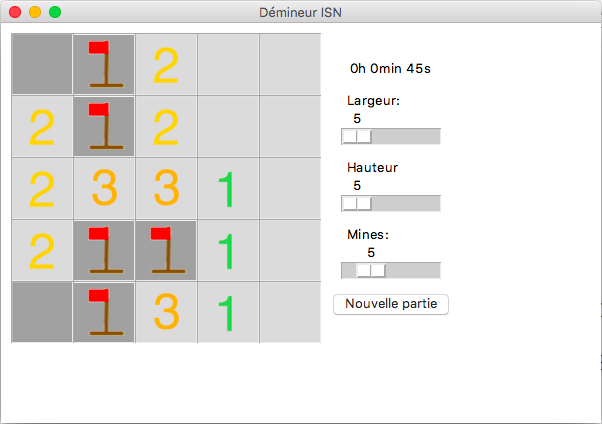
\includegraphics[scale=0.5]{presentation_projet.png}}
\newpage
\pagenumbering{roman}
\tableofcontents % Génère la table des matières ((sub)sub)sections
\newpage
\pagenumbering{arabic} % Passe la numérotation des pages en chiffres arabes

% CONTENU ---------------------------------------------------------------------

% SECTION ---------------------------------------------------------------------
\section{Présentation du projet}

\paragraph{Pourquoi ce projet ?}
Nous avons choisi de créer un démineur car, malgré son apparente simplicité,
ce n'est pas un jeu simple. En effet, il faut créer un générateur de terrain
qui soit le plus aléatoire et le plus rapide possible et qui place correctement
les numéros sur les cases. De plus, l'interface graphique associée doit
répondre à plusieurs évènements (clic sur le terrain ou non, clic gauche ou
droit, clic sur une case découverte ou non, ...).

\paragraph{Ce qui existait déjà:}
Nous avons effectué des recherches pour nous informer sur les solutions
existantes sur le Web (sur Github notamment). Nous avons trouvé au final assez
peu de ressources: nous cherchions principalement des sources graphiques pour
les éléments du jeu mais n'en n'avons pas trouvées et les avons faites à la
main. \\
Pour ce qui est du code, nous avons éviter de regarder ce qui avait déjà été
fait pour ne pas copier, surtout quand il s'agissait de code Python.

\paragraph{Ce que nous avons obtenu des recherches sur le Web:}
J'ai lu beaucoup de code sur Github, que ce soit en C, C++, C\# ou Java sur
Github afin d'avoir une idée de la logique derrière un démineur. Ce qui est
ressorti est qu'il existe tellement d'approches différentes qu'il y en a
quasiment une par projet. \\
Les codes lus étaient soit en anglais soit en français. J'ai trouvé des
exemples basés sur la programmation orienté objet, d'autres sur un paradigme
fonctionnel et enfin certains utilisaient des boucles évènementielles.

% ----------------------------------------------------------------- FIN SECTION

\newpage

% SECTION ---------------------------------------------------------------------
\section{Les idées et objectifs du projet}

% SUBsection ------------------------------------------------------------------
\subsection{Cahier des charges du projet}

\paragraph{}
Pour réaliser ce projet au mieux possible avec nos capacités nous avons choisi
de limiter la charge de travail. Ainsi ils existent de nombreuses améliorations
possibles pour notre démineur. Voici toutefois les idées qui nous ont servies
de base de départ.

\paragraph{}

\begin{itemize}
\item Génération d'un terrain miné aléatoire, de la taille demandée
(avec un taille minimum et maximum),
\item Adapter la taille des cases aux dimensions du terrains,
\item Pouvoir relancer une partie sans relancer l'application,
\item Pouvoir placer des drapeaux,
\item Avoir un chronomètre mesurant la durée de la partie,
\item Placer une mine de couleur différente des autres pour signaler celle qui
a fait perdre la partie, le cas échéant,
\item Afficher un message de fin de partie,
\item Pouvoir propager la révélation des cases si l'on clique sur une case sans
mines aux alentours ou pour révéler le terrain en fin de partie
\end{itemize}

% -------------------------------------------------------------- fin SUBsection

% SUBsection ------------------------------------------------------------------
\subsection{Moyens de réalisation du projet}

\paragraph{Choix du langage:}
Nous avons choisi d'utiliser le langage \emph{Python} en version 3.5. Ce choix
a été motivé par plusieurs raisons. La première raison était que nous avions
tous étudié ce langage au cours de l'année et le connaissions donc un minimum.
La seconde raison est la communauté Python, qu'elle soit française ou anglaise,
qui est très développée et active et donc plus à même de nous aider en cas
de problème important. La dernière raison était plus spécifique à notre groupe,
puisqu'elle vient du fait que j'ai déjà beaucoup codé en Python, que ce soit
pour des programmes graphiques ou en ligne de commande.

\paragraph{Choix du `type' de code:}
Nous avons choisi d'écrire du code sous forme de fonctions et en partant sur
une gestion évènementielle du démineur

% -------------------------------------------------------------- fin SUBsection

% ----------------------------------------------------------------- FIN SECTION

% SECTION ---------------------------------------------------------------------
\section{Organisation du travail en groupe}



% ----------------------------------------------------------------- FIN SECTION

% SECTION ---------------------------------------------------------------------
\section{Réalisation}



% ----------------------------------------------------------------- FIN SECTION

% SECTION ---------------------------------------------------------------------
\section{Intégration de ma partie}



% ----------------------------------------------------------------- FIN SECTION

% SECTION ---------------------------------------------------------------------
\section{Bilan du projet}



% ----------------------------------------------------------------- FIN SECTION

% ----------------------------------------------------------------- FIN CONTENU
\end{document}
